\documentclass[conference]{IEEEtran}
\IEEEoverridecommandlockouts
% The preceding line is only needed to identify funding in the first footnote. If that is unneeded, please comment it out.
\usepackage{cite}
\usepackage{amsmath,amssymb,amsfonts}
\usepackage{algorithmic}
\usepackage{graphicx}
\usepackage{textcomp}
\usepackage{xcolor}
\usepackage{listings}
\usepackage{hyperref}
\usepackage{tikz}
\usetikzlibrary{shapes.geometric, arrows, positioning, fit, backgrounds}

\def\BibTeX{{\rm B\kern-.05em{\sc i\kern-.025em b}\kern-.08em
    T\kern-.1667em\lower.7ex\hbox{E}\kern-.125emX}}

\begin{document}

\title{ExamCell: An Automated Exam Timetable Scheduling System Using Backtracking Constraint Satisfaction \\
{\footnotesize \textsuperscript{*}A Java Mini-Project Report}
}

\author{\IEEEauthorblockN{1\textsuperscript{st} Team Member}
\IEEEauthorblockA{\textit{Department of Computer Engineering} \\
\textit{MIT World Peace University}\\
Pune, India \\
member1@example.com}
\and
\IEEEauthorblockN{2\textsuperscript{nd} Team Member}
\IEEEauthorblockA{\textit{Department of Computer Engineering} \\
\textit{MIT World Peace University}\\
Pune, India \\
member2@example.com}
\and
\IEEEauthorblockN{3\textsuperscript{rd} Team Member}
\IEEEauthorblockA{\textit{Department of Computer Engineering} \\
\textit{MIT World Peace University}\\
Pune, India \\
member3@example.com}
\and
\IEEEauthorblockN{4\textsuperscript{th} Team Member}
\IEEEauthorblockA{\textit{Department of Computer Engineering} \\
\textit{MIT World Peace University}\\
Pune, India \\
member4@example.com}
}

\maketitle

\begin{abstract}
Scheduling examinations in educational institutions is a complex resource allocation problem often hindered by constraints such as room capacities, faculty availability, and student batch overlaps. This paper presents \textit{ExamCell}, an automated exam scheduling system developed using Java technologies. The system models the scheduling task as a Constraint Satisfaction Problem (CSP) and solves it using a recursive backtracking algorithm. The application architecture integrates a Java Swing-based desktop interface for administrative tasks, a MySQL database for persistence via JDBC, and a Servlet/JSP web layer for students to access the generated timetables. The system ensures conflict-free scheduling while adhering to strict resource constraints, demonstrating the practical application of object-oriented design, multithreading, and client-server architectures in a unified educational project.
\end{abstract}

\begin{IEEEkeywords}
Timetable Scheduling, Backtracking, Constraint Satisfaction Problem, Java, JDBC, Servlets
\end{IEEEkeywords}

\section{Introduction}
The manual generation of examination timetables is a tedious, error-prone task that educational institutions face every semester. The problem fundamentally revolves around allocating a set of events (exams) into a limited number of resources (time slots, classrooms, and faculty supervisors) such that no conflicts occur. Typical conflicts include assigning two exams for the same student batch at the same time, double-booking a classroom, or assigning a faculty member to invigilate multiple rooms simultaneously.

To address this challenge, we developed \textit{ExamCell}, a robust software solution tailored for academic environments. The objective of this project is twofold: first, to provide a functional and automated scheduling prototype; second, to demonstrate proficiency in core Java programming concepts as part of the laboratory curriculum. The system incorporates principles of Object-Oriented Programming (OOP), Multithreading, Database Connectivity (JDBC), and web deployment using Java Servlets and JSP.

\section{System Architecture}
The architecture of \textit{ExamCell} is designed as a multi-tier application, emphasizing separation of concerns while keeping the implementation concise enough for an educational prototype. The system comprises three primary layers:

\begin{itemize}
    \item \textbf{Data Layer}: A relational MySQL database storing information about Subjects, Classrooms, Faculty, Time Slots, and final Allocations.
    \item \textbf{Application Logic Layer}: A core engine written in standard Java that retrieves data, runs the scheduling algorithm, and returns the optimized timetable.
    \item \textbf{Presentation Layer}: A dual-interface approach featuring a desktop UI (Java Swing) for administrators and a web UI (JSP/HTML) for end-users (students and faculty).
\end{itemize}

\begin{figure}[htbp]
\centerline{
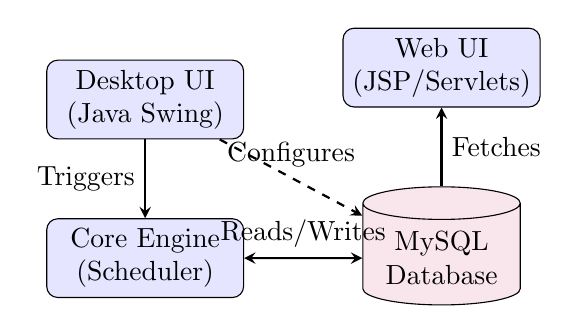
\begin{tikzpicture}[
    node distance=1.5cm,
    box/.style={draw, rounded corners, minimum width=2.5cm, minimum height=1cm, align=center, fill=blue!10},
    db/.style={draw, cylinder, shape border rotate=90, aspect=0.25, minimum width=2cm, minimum height=1.5cm, align=center, fill=purple!10},
    arrow/.style={thick,->,>=stealth}
]
    % Nodes
    \node[box] (admin) {Desktop UI \\ (Java Swing)};
    \node[box, below=1cm of admin] (engine) {Core Engine \\ (Scheduler)};
    \node[db, right=1.5cm of engine] (db) {MySQL \\ Database};
    \node[box, above=1cm of db] (web) {Web UI \\ (JSP/Servlets)};
    
    % Arrows
    \draw[arrow] (admin) -- node[left] {Triggers} (engine);
    \draw[arrow,<->] (engine) -- node[above] {Reads/Writes} (db);
    \draw[arrow] (db) -- node[right] {Fetches} (web);
    \draw[arrow, dashed] (admin) -- node[above] {Configures} (db);

\end{tikzpicture}
}
\caption{ExamCell Multi-Tier System Architecture}
\label{fig:architecture}
\end{figure}

The entities within the system are modeled using encapsulation, forming the domain models (`Subject`, `Classroom`, `Faculty`, `TimeSlot`, `Allocation`). The data persistence layer is handled by a unified `DatabaseHelper` class that manages all JDBC connections and queries.

\section{Methodology and Implementation}

\subsection{Problem Formulation as a CSP}
The scheduling problem is modeled as a Constraint Satisfaction Problem (CSP). A CSP consists of a set of variables, a domain of values for each variable, and a set of constraints restricting the allowable combinations of values.
In \textit{ExamCell}, the variables are the examinations (Subjects), and the domain is the Cartesian product of available Time Slots, Classrooms, and Faculty. 

The constraints are defined as follows:
\begin{enumerate}
    \item \textbf{Room Availability}: A room can host only one exam per time slot.
    \item \textbf{Faculty Availability}: A faculty member can invigilate only one room per time slot.
    \item \textbf{Batch Overlap}: Two subjects belonging to the same department and semester cannot be scheduled in the same time slot.
    \item \textbf{Capacity Constraint}: The assigned classroom's capacity must be greater than or equal to the estimated number of students for the subject.
\end{enumerate}

\subsection{Backtracking Algorithm}
To solve the CSP, the system utilizes a Depth-First Search (DFS) with backtracking. The algorithm attempts to build a schedule incrementally. If a partial schedule violates any constraints, the algorithm abandons it ("backtracks") and tries alternative assignments.

The implementation involves an abstract base class `Scheduler` and a concrete subclass `BacktrackingScheduler`. The `solve` function iterates recursively:
\begin{enumerate}
    \item Select the next unscheduled subject.
    \item Iterate through all possible combinations of Time Slots, Classrooms, and Faculty.
    \item Validate the combination against the predefined constraints using the `isValid()` method.
    \item If valid, tentatively add the allocation to the current schedule and recursively call `solve()` for the next subject.
    \item If the recursive call returns false (indicating a dead-end), remove the tentative allocation and continue the loop.
    \item If all combinations fail, return false to trigger backtracking in the parent call.
\end{enumerate}

\begin{figure}[htbp]
\centerline{
\resizebox{0.48\textwidth}{!}{
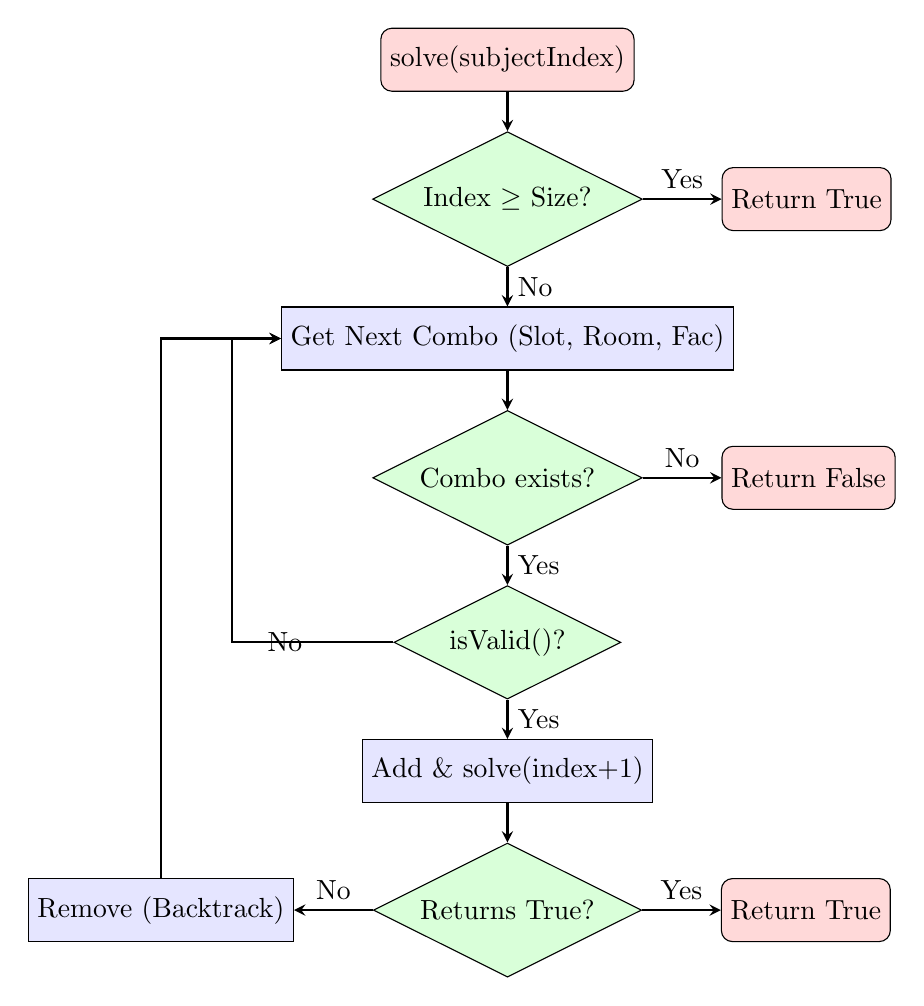
\begin{tikzpicture}[
    node distance=1cm,
    startstop/.style={rectangle, rounded corners, minimum width=2cm, minimum height=0.8cm, text centered, draw=black, fill=red!15},
    process/.style={rectangle, minimum width=2.5cm, minimum height=0.8cm, text centered, draw=black, fill=blue!10},
    decision/.style={diamond, aspect=2, minimum width=2.5cm, minimum height=0.8cm, text centered, draw=black, fill=green!15},
    arrow/.style={thick,->,>=stealth}
]
    % Nodes
    \node (start) [startstop] {solve(subjectIndex)};
    \node (base) [decision, below=0.5cm of start] {Index $\ge$ Size?};
    \node (rettrue1) [startstop, right=1cm of base] {Return True};
    
    \node (loop) [process, below=0.5cm of base] {Get Next Combo (Slot, Room, Fac)};
    \node (checkcombo) [decision, below=0.5cm of loop] {Combo exists?};
    \node (retfalse) [startstop, right=1cm of checkcombo] {Return False};
    
    \node (valid) [decision, below=0.5cm of checkcombo] {isValid()?};
    
    \node (recurse) [process, below=0.5cm of valid] {Add \& solve(index+1)};
    \node (success) [decision, below=0.5cm of recurse] {Returns True?};
    \node (rettrue2) [startstop, right=1cm of success] {Return True};
    
    \node (backtrack) [process, left=1cm of success] {Remove (Backtrack)};

    % Arrows
    \draw [arrow] (start) -- (base);
    \draw [arrow] (base) -- node[above] {Yes} (rettrue1);
    \draw [arrow] (base) -- node[right] {No} (loop);
    
    \draw [arrow] (loop) -- (checkcombo);
    \draw [arrow] (checkcombo) -- node[above] {No} (retfalse);
    \draw [arrow] (checkcombo) -- node[right] {Yes} (valid);
    
    \draw [arrow] (valid) -- node[right] {Yes} (recurse);
    \draw [arrow] (valid) -- node[left] {No} ++(-3.5,0) |- (loop);
    
    \draw [arrow] (recurse) -- (success);
    \draw [arrow] (success) -- node[above] {Yes} (rettrue2);
    \draw [arrow] (success) -- node[above] {No} (backtrack);
    
    \draw [arrow] (backtrack) |- (loop);

\end{tikzpicture}
}
}
\caption{Backtracking Algorithm Flowchart}
\label{fig:flowchart}
\end{figure}

\subsection{Multithreading and UI Responsiveness}
Due to the combinatorial explosion inherent in CSPs, the backtracking algorithm can be computationally intensive. To ensure the Java Swing desktop application remains responsive, the scheduling process is executed on a background thread. 
Upon completion, the background thread uses `SwingUtilities.invokeLater()` to safely update the table models on the Event Dispatch Thread (EDT) and save the successful allocations back to the database.

\subsection{Web Deployment}
A Servlet (`ViewTimetableServlet`) handles HTTP GET requests, connects to the database via `DatabaseHelper` to execute a multi-table SQL `JOIN` query, and retrieves the generated timetable. The data is then forwarded to a JavaServer Page (`index.jsp`) for dynamic HTML rendering, providing a clean interface for students.

\section{Results and Discussion}
The system was tested using a sample dataset consisting of 6 subjects across two departments (Computer Science and Information Technology), 3 classrooms, 4 faculty members, and 4 time slots.

Upon execution, the backtracking algorithm successfully navigated the search space and generated a conflict-free timetable. The constraints were rigorously enforced:
\begin{itemize}
    \item No two CS Semester 6 subjects were placed in the same time slot.
    \item IT and CS exams were allowed to occur simultaneously in different rooms, provided the rooms and faculty were distinct, demonstrating the efficiency of the batch conflict logic.
    \item The desktop application successfully exported the generated schedule to a structured text file using Java's `BufferedWriter`.
\end{itemize}

The integration of JDBC proved reliable in persisting the data, allowing the web interface to display real-time updates immediately after the administrator generated the schedule.

\section{Conclusion}
The \textit{ExamCell} project successfully implements an automated exam scheduling system, fulfilling both functional requirements and educational objectives. By employing a backtracking constraint satisfaction algorithm, the system effectively resolves scheduling conflicts while adhering to strict resource limitations. The project structure seamlessly integrates core Java concepts—including object-oriented design, multithreading, database connectivity, and servlet-based web development—into a cohesive, multi-tier application. Future enhancements could include implementing heuristic-based optimizations (such as the Minimum Remaining Values heuristic) or genetic algorithms to improve performance on significantly larger datasets.

\begin{thebibliography}{00}
\bibitem{b1} R. Dechter, \textit{Constraint Processing}, Morgan Kaufmann, 2003.
\bibitem{b2} S. Russell and P. Norvig, \textit{Artificial Intelligence: A Modern Approach}, 3rd ed. Prentice Hall, 2009.
\bibitem{b3} Oracle, ``Java SE Documentation,'' [Online]. Available: https://docs.oracle.com/en/java/javase/
\bibitem{b4} MySQL, ``MySQL Connector/J Developer Guide,'' [Online]. Available: https://dev.mysql.com/doc/connector-j/en/
\end{thebibliography}

\end{document}
